\section{Développement firmware}
Dans cette section, nous allons décrire et expliquer le procédé de programmation du code qui a été implémenté dans le microcontrôleur PIC32MX130F256D.
Le processus de programmation du code dans le PIC32MX130F256D implique plusieurs étapes. Tout d'abord, il est nécessaire de disposer d'un environnement de développement intégré (IDE) adapté à ce microcontrôleur, ici, MPLAB X IDE, avec l'environnement Harmony permettant l'utilisation d'un configurateur graphiques pour les différentes libraires du PIC.

\subsection{Configuration des PINs dans Harmony}
{
	\begin{figure}[h]
		\centering
		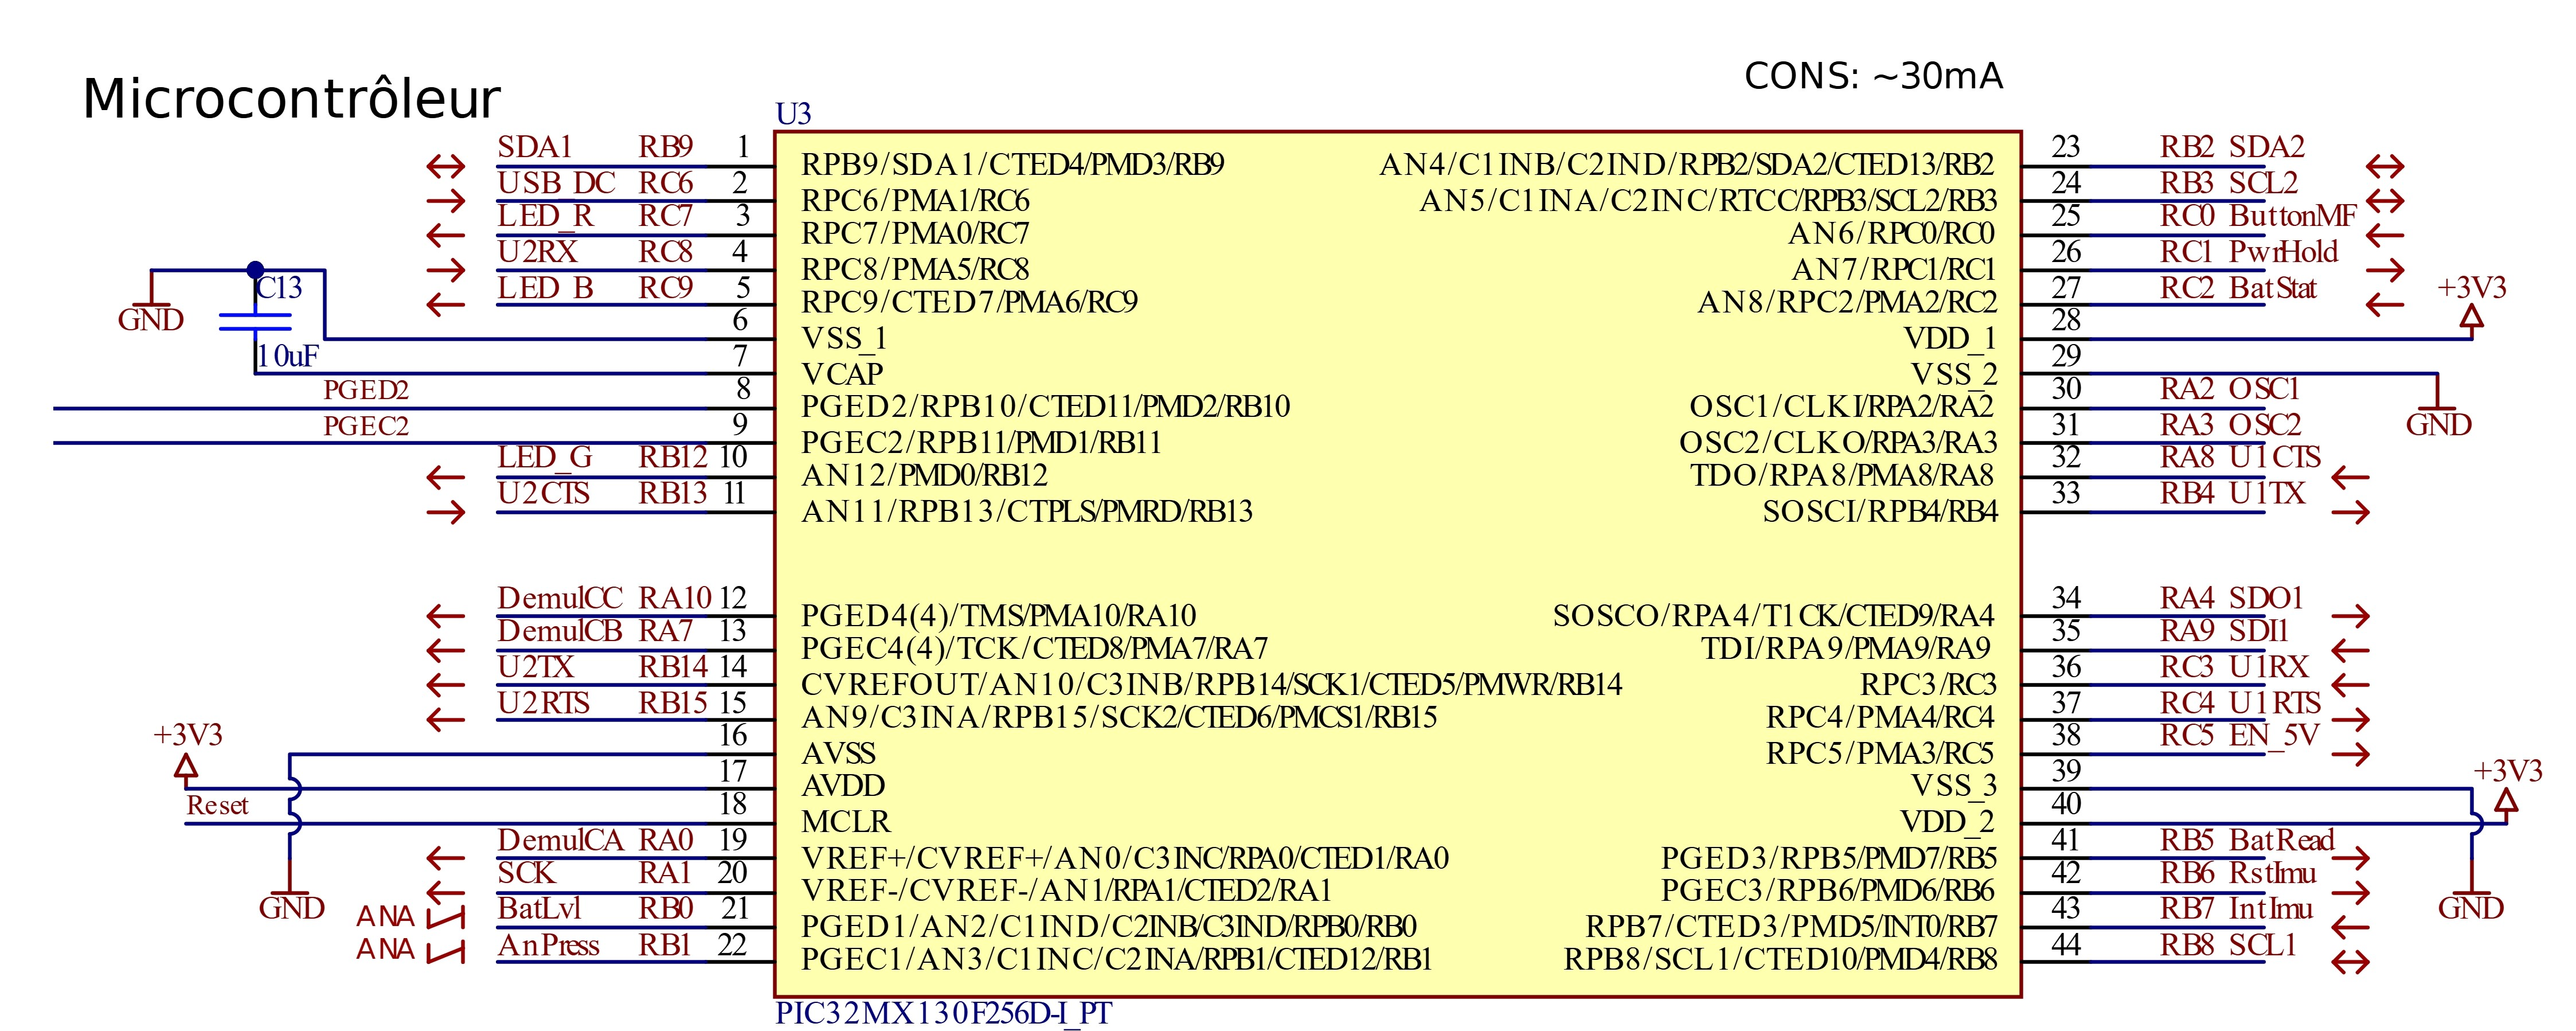
\includegraphics[width=.9\textwidth]{Figures/Dev-SOFT/MCU-Altium}
		\caption{Pinning réelles dans altium designer}
		\label{fig:mcu-altium}
	\end{figure}
	\begin{figure}[h]
		\centering
		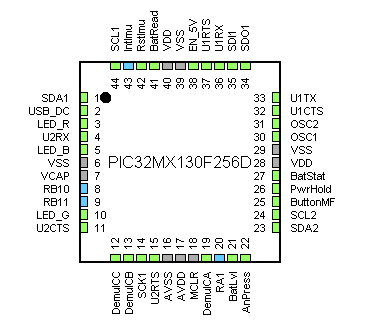
\includegraphics[width=0.5\textwidth]{Figures/Dev-SOFT/MCU-Harmony}
		\caption{Pinning dans Harmony}
		\label{fig:mcu-harmony}
	\end{figure}
	
	On peut voir que la PIN 20 (SCK) est en haute impédance dans harmony, tandis que la PIN14 qui était supposée être \textit{U2TX} est devenue SCK, ceci étant dû à une erreur : SCK n'est que valable sur la PIN14, il a donc fallut ajouter un fil extérieur pour router Pin14 à Pin20, sacrifiant ainsi la communication USB sur l'UART2, cette modification sera décrite ultérieurement.
	
	
}

\subsection{Configuration des périphériques dans Harmony}
{
	\paragraph{Timers :} Deux timers seront utilisés, l'un pour mesurer des attentes en ms et l'autre moins rapide, pour les diverses actions du programmes, avec une interruptions chaque 10ms.
	\begin{table}[h]
		\centering
		\begin{tabular}{|l|l|}
			\hline
			Timer & Temps voulu \\
			\hline
			Timer 1 & 1ms \\
			\hline
			Timer 2 & 10ms \\
			\hline
		\end{tabular}
	\end{table}
	
	\begin{figure}[h]
		\centering
		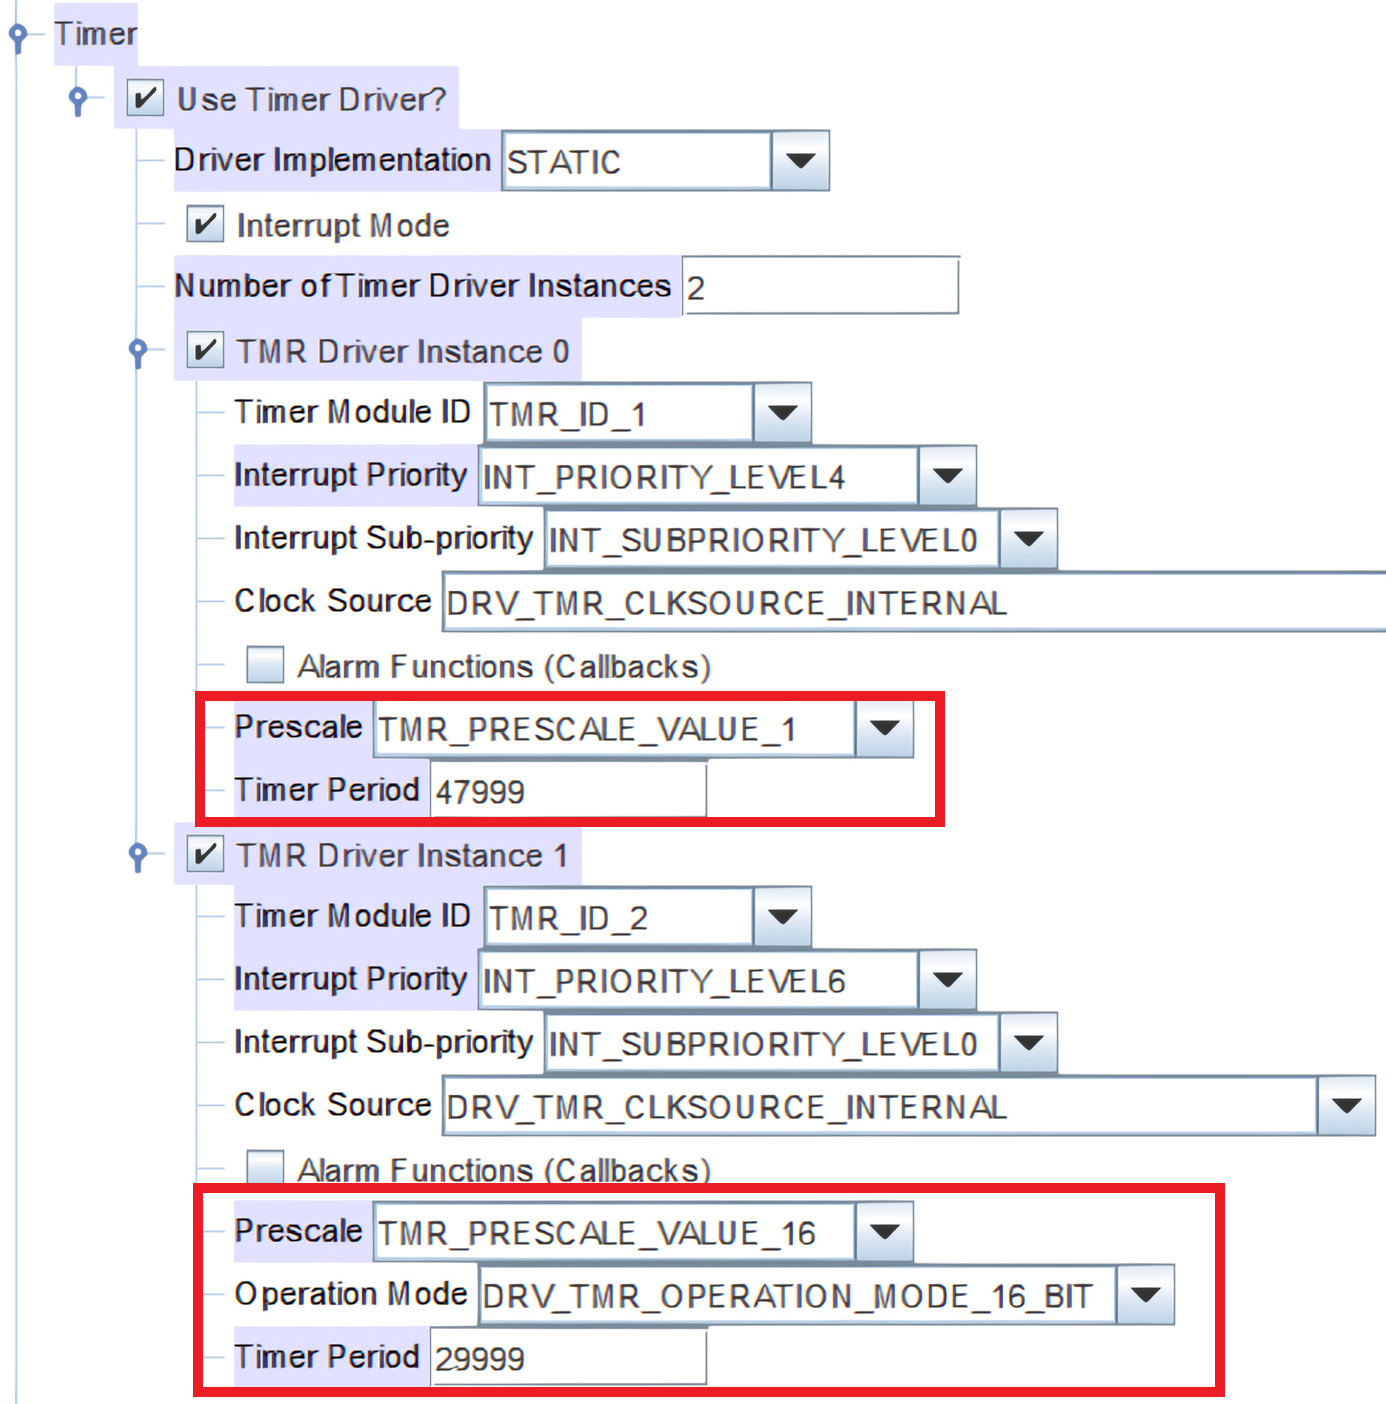
\includegraphics[width=0.7\linewidth]{Figures/Dev-SOFT/Timer_config}
		\caption{}
		\label{fig:timerconfig}
	\end{figure}
	
	
	\paragraph{USART :} 
	
	\paragraph{Carte SD - SPI :} ASDASDASD

}
